\documentclass{template}

\graphicspath{{../figures/}{logos/}}

%--------------------------------------

\titre{Palimpsest}
\soustitre{A Skill-Extensible Agentic Workflow for\\
Provenance-Tracked, Ontology-Aligned Extraction\\
of Structured Data from the Scientific Literature
\\[0.8cm]
{\normalsize\normalfont MSc Mini-Thesis in Materials Engineering · RWTH Aachen University\\
Interim Report / Working Draft}}
\eleves{Rakibuzzaman Rahat}
\enseignant{[matriculation no.]}
\datevar{May 2026}

%--------------------------------------

\begin{document}

\fairepagedegarde

\fairetabledesmatieres

%--------------------------------------

\begin{abstract}
Quantitative results across the experimental sciences are reported predominantly as prose, tables, and figures within PDF articles, where they remain findable as documents but not as reusable data. Comparing a measured quantity across even a modest set of papers therefore requires manual re-reading of each one. This report describes palimpsest, an agent workflow that reads a collection of research PDFs and produces a queryable, provenance-tracked, ontology-aligned RDF knowledge graph. The quantities to be extracted in a given field are not encoded in the agent; they are supplied by a \textit{skill}, a self-contained specification of the field's quantities and conventions together with an ontology-aligned schema, so that a new domain is added by authoring a skill rather than by modifying the agent. The agent is otherwise deliberately minimal: a tool-using language model loop rather than a general agent framework. Every extracted value is recorded as a provenance-bearing object traceable to the page region from which it was read. We develop and evaluate the system on one demonstrator domain, energy-materials electrocatalysis: the oxygen evolution reaction (OER) and proton-exchange-membrane (PEM) water electrolysis. Our first empirical study compares five state-of-the-art PDF parsers, evaluated not only on transcription fidelity but on downstream extraction accuracy: the accuracy with which a fixed language model recovers the intended measurements from each parser's output. This document presents the problem, related work, the system design, and the planned evaluation methodology. The agent loop, the parsing infrastructure, and the cost controls are implemented; the schema, extraction, and viewer components are specified and under active development, and the parser comparison is in progress. No comparative results are reported, as none have yet been produced. This is a methodological proposal supported by a working foundation.
\end{abstract}

%--------------------------------------

\section{Introduction}

\subsection{Problem statement}

Across the experimental sciences, the quantitative content of a paper is presented for human readers rather than for machine processing. That content comprises the measured values, the conditions under which they were obtained, and the materials or systems described. A given result is typically stated once in the text, repeated in a table, and shown in a figure, under names and units that vary between research groups. For a single paper this poses no difficulty; the difficulty lies in aggregation. Questions that span many papers, such as identifying which reported system performs best under comparable conditions, require substantial manual effort, because no shared, machine-actionable record of each paper's measurements exists.

We use one field as a running demonstrator: energy-materials electrocatalysis, and specifically the oxygen evolution reaction (OER) and PEM water electrolysis. We take it as representative rather than special. A single OER study reports a cluster of figures of merit such as the overpotential required to reach a current density of 10 mA cm$^{-2}$, the Tafel slope in millivolts per decade, the exchange current density, the electrochemically active surface area (ECSA), the mass activity, the turnover frequency, and a stability figure in hours, each qualified by its measurement conditions: the electrolyte and its pH, the potential referenced to the reversible hydrogen electrode, the scan rate, whether the data were \textit{iR}-corrected, and whether a rotating-disc electrode or a full membrane-electrode assembly was used. The same quantity may be named differently across papers and located variously in running text, in a table cell, or only in a plotted Tafel curve. Consequently, a question as routine as which iridium-oxide catalyst reaches the lowest overpotential at 10 mA cm$^{-2}$ in acid cannot be answered without reading each paper individually. This difficulty is not specific to electrocatalysis; it characterises the quantitative literature of most experimental fields, which motivates a design that is not tied to a single domain.

\begin{figure}[H]
    \centering
    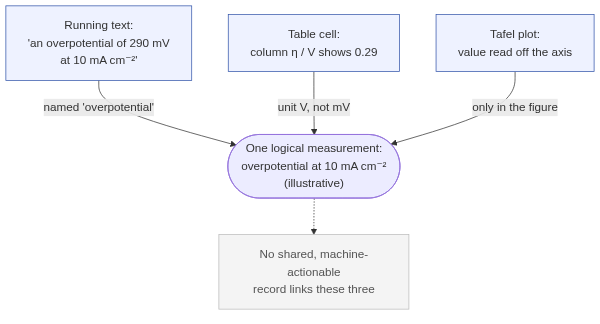
\includegraphics[width=0.88\textwidth]{scattered-quantity.png}
    \caption{The same logical measurement scattered across a paper's text, a table, and a figure under different names, units, and locations, with no shared machine-actionable record linking them. Values are illustrative.}
    \label{fig:scattered}
\end{figure}

These characteristics correspond to the gap addressed by the FAIR principles, under which data should be Findable, Accessible, Interoperable, and Reusable, including reusable by machines and not only by human readers (Wilkinson et al., 2016). Measured against this standard, the quantitative content of the primary literature is largely non-compliant: the measurements are findable as PDFs but not as data, are not interoperable because they lack a shared vocabulary, and are not reusable without human intervention for each value.

This deficiency matters because quantitative data are the input to data-driven materials research. Accelerated materials design is the use of computation, machine learning, and high-throughput methods to shorten the discovery and optimisation of materials. It depends on large, consistent, machine-readable property datasets to train models, parameterise simulations, and prioritise experiments (de Pablo et al., 2019; Butler et al., 2018), and the largest underused source of such data is the published literature itself. A pipeline that converts papers into curated, unit-normalised, ontology-aligned, provenance-bearing data therefore sits at the front of this workflow, supplying the data layer on which later analysis, simulation, and experiment depend. This need is not specific to materials: extraction, curation, and reuse with full traceback are foundational to any data-driven scientific system.

\subsection{Aim and scope}

Palimpsest aims to render this content FAIR retrospectively, one corpus at a time, using a small and auditable tool. The system converts a collection of research PDFs into an RDF knowledge graph in which each measurement is an ontology-aligned node carrying its units, its experimental conditions, and a complete provenance record. The objective is not extraction in isolation but data fit for downstream use: values whose units, conditions, and provenance are explicit enough to be filtered, compared, and used as inputs to analysis, simulation, or experiment, with the provenance record allowing a researcher to verify a value before relying on it. The agent is domain-agnostic: the quantities to extract in a given field are supplied externally, through a skill that specifies the field's quantities and conventions together with an ontology-aligned schema, so that extending the system to a new domain requires authoring a skill rather than modifying the agent (Section 4.3). The intended mode of use is interactive: the user directs the agent at a paper or a collection of papers, requests the quantities of interest, inspects the extracted output, and corrects it where required. Because the agent is built directly on the model providers' SDKs rather than on a hosted product, the model and provider can be changed at run time, each call is metered against a fixed budget, and the full pipeline remains inspectable and modifiable. The remainder of this report presents the design in general terms and grounds each component in the electrocatalysis demonstrator.

\subsection{Contributions}

This mini thesis makes four contributions, stated here as objectives and developed in Section 4:

\begin{enumerate}
\item A general, skill-extensible agentic workflow for extracting structured data from research papers: a minimal tool-using loop with interchangeable model backends and a fixed cost ceiling, in which each scientific domain is supplied by a self-contained skill and an ontology-aligned schema rather than by additional code.
\item A parser comparison: a domain-general evaluation method, demonstrated first on the electrocatalysis corpus. Its principal metric is downstream extraction accuracy conditional on the parser, the accuracy with which a fixed language model recovers the target measurements from each parser's output, as distinct from transcription fidelity.
\item An ontology-aligned, provenance-complete data model based on EMMO, QUDT, and PROV-O, including, for the demonstrator domain, a preliminary, documented analysis of where the EMMO electrochemistry domain appears to lack terms required for OER.
\item A schema strategy that also serves as a skill-creation method: a comparison of schema-first and explore-first extraction, and a hybrid in which exploration of a new corpus yields a derived schema and heuristics that are packaged into the corresponding domain skill.
\end{enumerate}

%--------------------------------------

\section{Background and related work}

\subsection{Document parsing}

Conversion of a scientific PDF into structured text is an active research problem, and several distinct approaches are now available. We group them into three design families, and our comparison set spans all three.

The first family is the classical computer-vision pipeline: a sequence of specialised, comparatively small models for layout detection, text detection and recognition, table-structure recognition, and formula parsing. PaddleOCR is a mature representative; its PP-StructureV3 solution composes sub-100-million-parameter models for layout analysis, the PP-OCRv5 detector and recogniser, and table-structure recognition, and reports accuracy competitive with substantially larger vision-language models at lower computational cost (PaddleOCR Team, 2025). IBM's docling is adjacent to this family, pairing layout analysis with the TableFormer table-structure model in a self-contained, MIT-licensed pipeline that converts PDFs to structured JSON or Markdown and recovers reading order and table cells (Auer et al., 2024). Recent releases deliver this functionality through the compact granite-docling-258M model, the variant we deploy.

The second family is the decoupled, two-stage vision-language model, which separates global layout analysis from local transcription. MinerU2.5 is representative: a 1.2-billion-parameter model that first analyses layout on a downsampled image and then recognises content on native-resolution crops, confining high-resolution processing to the regions that require it (Niu et al., 2025).

The third family is the unified single-model parser, in which one vision-language model performs layout detection, OCR, and formula and table parsing together, typically by prompt switching, and emits per-element bounding boxes alongside text. dots.ocr (rednote-hilab, 2025) is a compact ($\sim$1.7-billion-parameter), MIT-licensed example, and Chandra (Datalab, 2026) is a vision-language OCR model targeting complex tables, forms, and handwriting with full layout recovery. The Allen Institute's olmOCR also belongs to this family: a single fine-tuned 7-billion-parameter model optimised for large-scale, low-cost batch linearisation (Poznanski et al., 2025). We assessed olmOCR during parser selection but excluded it on practical deployment grounds (Section 6.4), and include it here only as related context.

While the effect of parser and OCR quality on downstream tasks is recognised in general, the literature does not provide a task-grounded comparison of these systems for quantitative extraction on a specific scientific subdomain. The respective projects report results on general document-parsing benchmarks, which measure transcription against reference text but do not measure whether the output is adequate for a downstream model to recover, for example, a Tafel slope and associate it with the correct current-density range. Providing such a comparison for the OER literature, scored at the level of individual measurement records, is the empirical core of this work's parser study.

\subsection{Extracting structured data from scientific text}

Information extraction from the materials literature predates large language models, but these models have substantially reduced its cost. Dunn et al. (2022) showed that a fine-tuned general language model can perform joint named-entity and relation extraction over hierarchical materials-chemistry text and emit structured JSON directly. Polak and Morgan (2024) addressed robustness with ChatExtract, a conversational prompting protocol that extracts candidate values and then verifies them through follow-up questions, reporting precision and recall above 90\% and 80\% respectively on materials-property data with limited task-specific engineering.

Two findings from this literature inform our design. First, extraction accuracy depends less on a single prompt than on a disciplined loop that validates, re-queries, and rejects low-confidence output. Second, extraction quality is bounded by the quality of the text supplied to the model: if a parser corrupts a table or omits a superscript, subsequent prompting cannot recover the lost value. The second finding is our reason for treating the parser as an experimental variable rather than as a fixed preprocessing step.

\subsection{Ontologies, units, and provenance}

For the extracted data to be interoperable rather than merely structured, it must be aligned to shared vocabularies. We build on three. The Elementary Multiperspective Material Ontology (EMMO) provides an upper- and domain-level ontology for materials science, including an electrochemistry domain that formalises concepts such as overpotential, electrocatalyst, and the Butler--Volmer relation (Del Nostro et al., 2024). QUDT (Quantities, Units, Dimensions and Types) provides machine-actionable IRIs for the units in which these quantities are expressed (QUDT, n.d.). The PROV Ontology (PROV-O), a W3C Recommendation, provides a domain-neutral model of provenance as relations among entities, activities, and agents (Lebo et al., 2013), which we use to record how each datum was produced.

These vocabularies are bound together at the schema level by LinkML, a data-modelling language designed to produce FAIR, ontology-ready data from a single human-readable definition, generating validation artefacts and JSON-LD contexts from one YAML source (Moxon et al., 2021). LinkML allows us to maintain the schema in one place while emitting the several machine representations the pipeline requires.

\subsection{Agentic workflows}

The system is an agent: a language model operating in a loop, with the ability to call tools and observe their results. A common approach is to adopt an agent-orchestration framework; we do not. The architecture follows the minimal pattern described by Ball (2025): a model, a loop, a set of tools, and sufficient context. We adopt it on the grounds that, at the scale of this project, a framework's control-flow abstractions add opacity without commensurate benefit. Section 4.1 sets out this choice in detail.

The one structural convention we adopt is the skill: a folder containing a concise, self-contained description of a task, which the agent discovers from its metadata and loads in full only when it is relevant. This is the progressive-disclosure pattern described by Anthropic (2025). Skills provide domain-specific competence to a domain-agnostic loop without enlarging the codebase, and they are our mechanism for supporting new fields; Section 4.3 develops them.

\subsection{Data-driven materials design}

The motivation for structured extraction is its role in data-driven materials research. The Materials Genome Initiative and subsequent work established computation and shared data as a route to faster materials discovery (de Pablo et al., 2019), and machine-learning methods now use curated property datasets to predict materials behaviour and to guide search (Butler et al., 2018). More recently, autonomous or self-driving laboratories have begun to close the loop between prediction and experiment, selecting and executing the next measurement automatically (Abolhasani \& Kumacheva, 2023). A constraint common to these approaches is the supply of trustworthy, machine-readable data: models must be trained, simulations parameterised, and candidates prioritised from property values that are consistent, unit-resolved, and traceable. Much of that data exists only in the prose, tables, and figures of the primary literature, which is the source palimpsest is built to convert.

\subsection{Summary of the gap}

In summary, existing work provides strong parsers but no task-grounded comparison of them on a scientific subdomain; effective LLM extraction methods that nonetheless assume clean input and rarely treat the parser as a variable; and mature ontologies for electrochemistry, units, and provenance, but limited tooling that binds an end-to-end extraction pipeline to all three while maintaining a complete provenance trail. Tooling that does so in a domain-agnostic manner, where supporting a new field requires authoring a skill rather than rewriting the extractor, is likewise lacking. Palimpsest addresses this gap.

%--------------------------------------

\section{The demonstrator domain and its target quantities}

The system is general but must be evaluated on a concrete corpus. Our demonstrator is energy-materials electrocatalysis: a reference corpus of PEM-electrolyser and acidic-OER catalyst papers, covering the chemistry of iridium- and ruthenium-oxide anodes and related materials, a field surveyed by Carmo et al. (2013). A development set of about 5 papers is used to author the schema and the OER skill, through the hybrid process of Section 4.3. The parser comparison is then run on a held-out evaluation corpus of about 25 papers from the same domain. We selected this corpus because it is dense, table-heavy, and quantitatively demanding, and therefore a stringent test of the pipeline. The same machinery applies to other fields once each is described by its own skill and schema (Section 4.3). For the electrocatalysis demonstrator, the system targets a defined set of figures of merit and their qualifying conditions:

\begin{itemize}
\item \textbf{Overpotential}, typically at a stated current density, following the 10 mA cm$^{-2}$ benchmarking convention for rotating-disc measurements (McCrory et al., 2013) or 1--2 A cm$^{-2}$ for full cells;
\item \textbf{Tafel slope}, in mV per decade, with the current-density range used for the fit;
\item \textbf{Exchange current density} and \textbf{charge-transfer coefficient};
\item \textbf{ECSA}, \textbf{mass activity}, and \textbf{turnover frequency};
\item \textbf{Stability}, in hours, at a stated current density and cell type.
\end{itemize}

Each figure of merit is meaningful only in conjunction with its conditions, so the data model treats a measurement and its conditions as a single unit (Section 4.3). The demonstrator vocabulary is deliberately narrow: a tightly scoped set of quantities makes reliable extraction and a meaningful ontology alignment achievable within our mini thesis. This narrowness reflects the scope of a single skill, the unit from which further fields are added, rather than a constraint built into the agent.

%--------------------------------------

\section{System design and methodology}

This section presents the system design and the planned evaluation methodology. Figure 2 shows the end-to-end pipeline, and the subsections that follow describe each component in turn.

\begin{figure}[H]
    \centering
    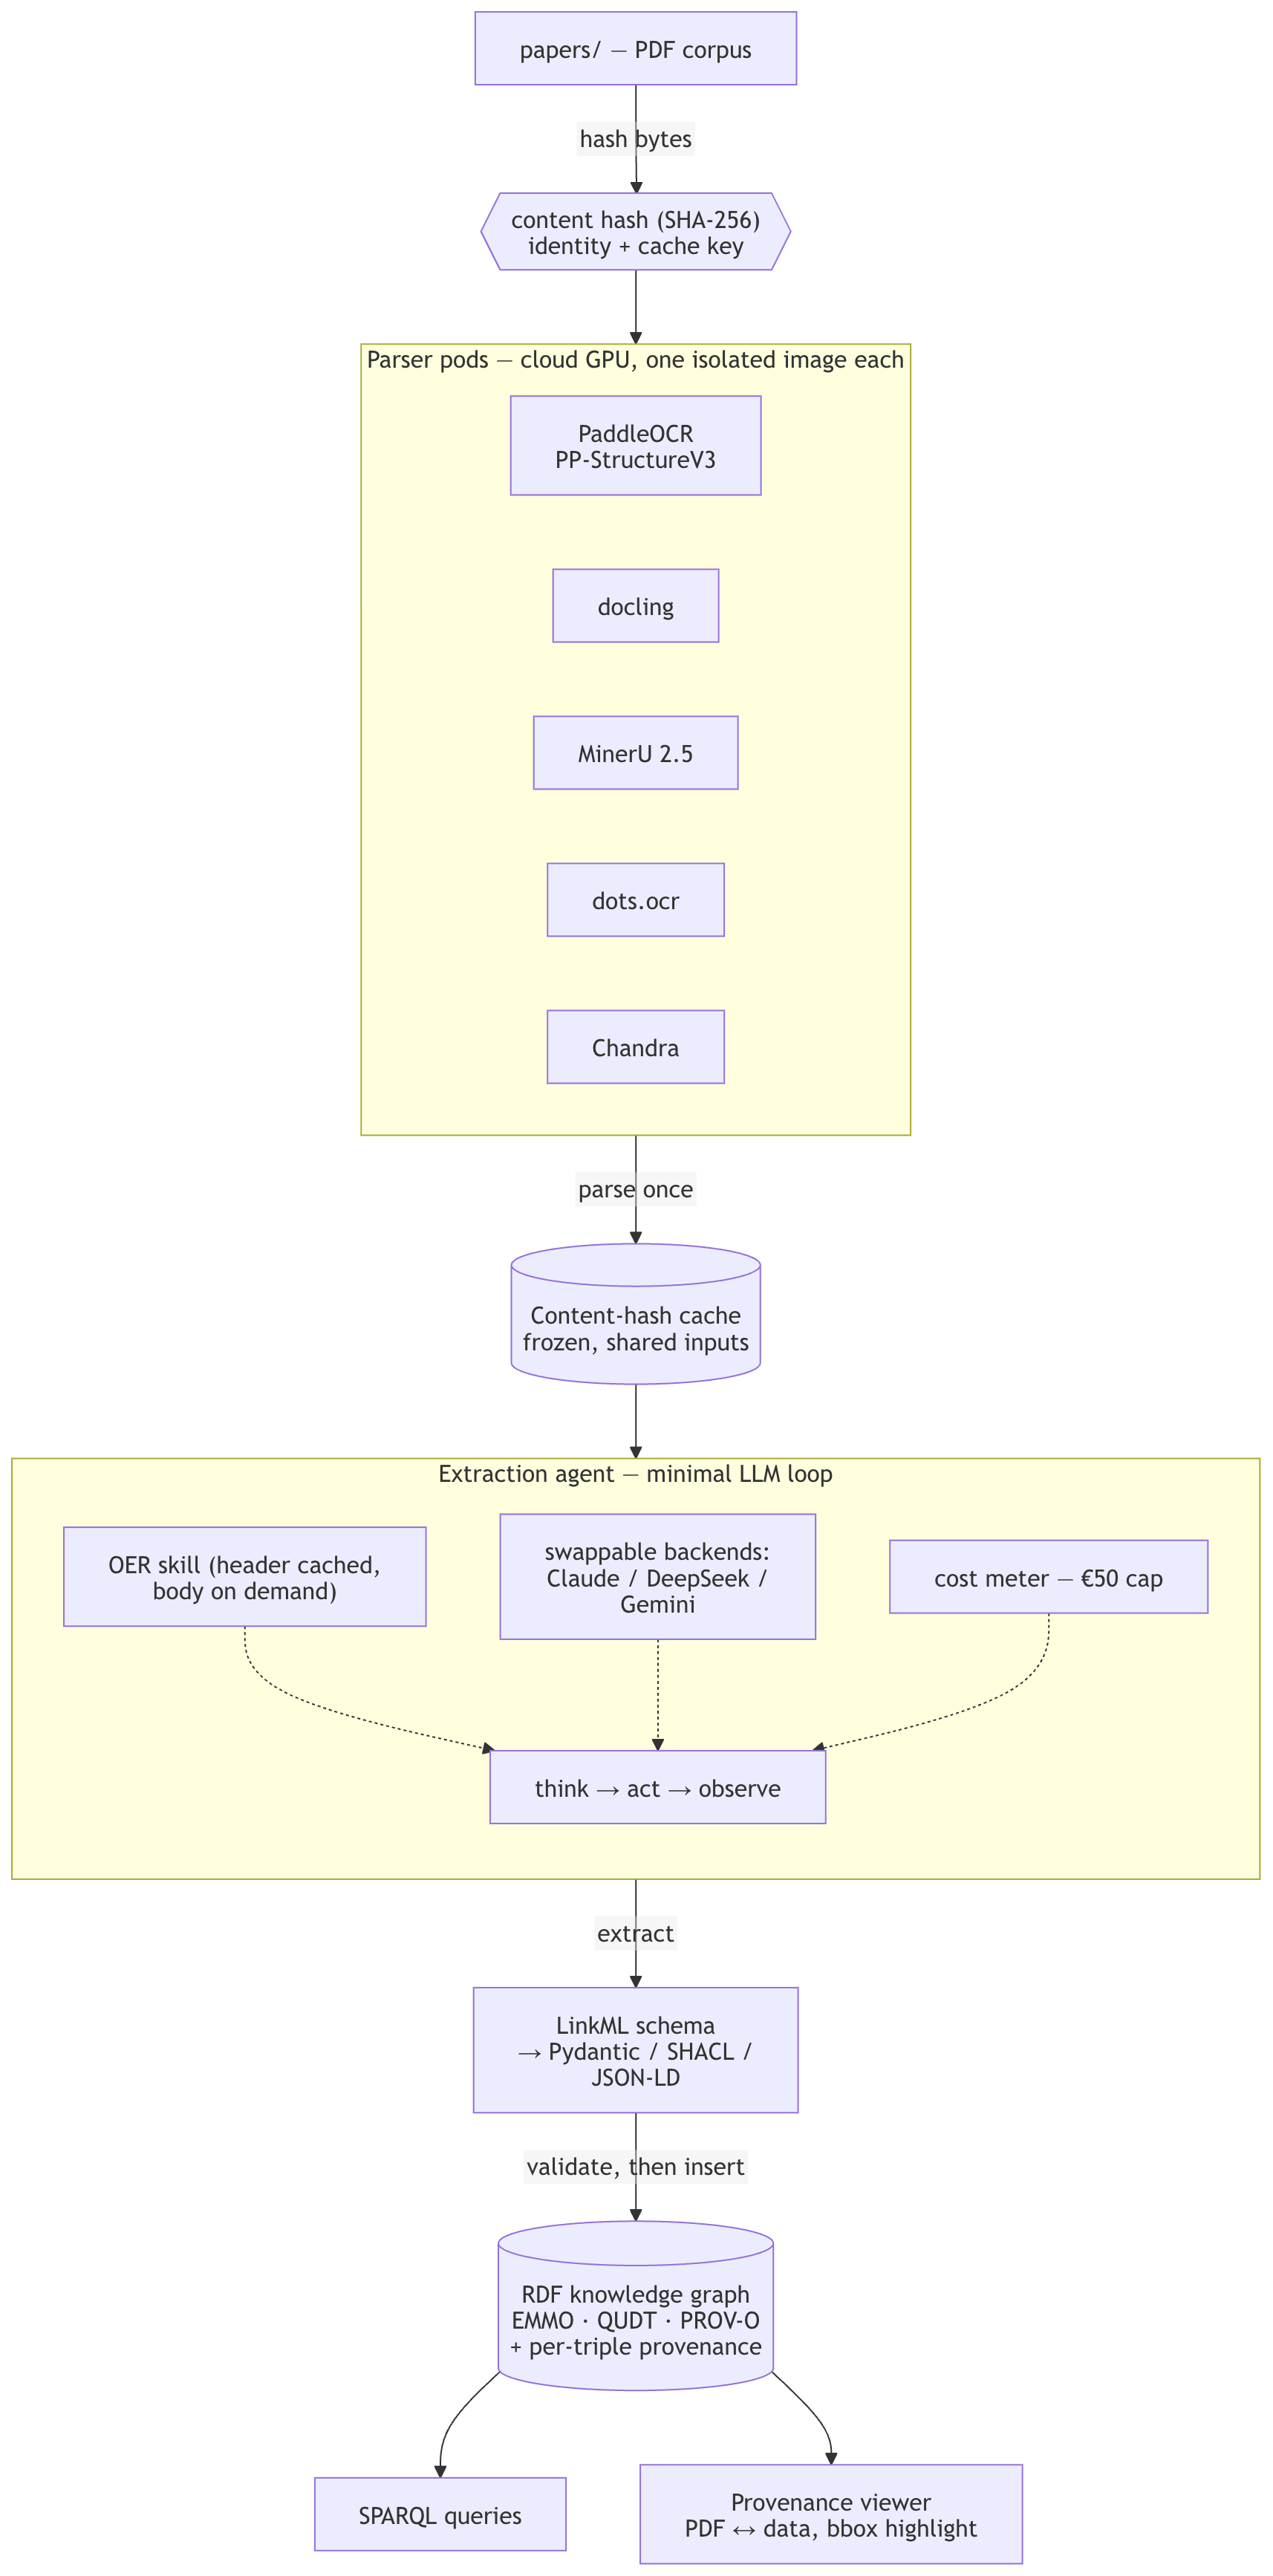
\includegraphics[width=0.5\textwidth]{architecture.png}
    \caption{End-to-end pipeline. A PDF is hashed once, parsed by each of the five parsers on isolated GPU pods, and cached; the extraction agent reads cached output, extracts and validates measurements against the LinkML schema, and writes them, with full provenance, into the ontology-aligned RDF graph, which is then queryable by SPARQL and inspectable in the viewer. The cost meter and interchangeable model backends gate the agent's loop. The agent itself is domain-agnostic: the loaded skill (here, OER extraction) and its schema supply the domain, so substituting the skill retargets the same pipeline at another field.}
    \label{fig:architecture}
\end{figure}

\subsection{Agent architecture}

At its core, palimpsest is a single loop. The agent reads user input; a slash command (\texttt{/cost}, \texttt{/budget}, \texttt{/model}) is dispatched directly, while any other input is appended to the conversation and sent to the language model together with a cached system prompt and a set of tool definitions. The model responds, the agent records the cost of the call, and any tool calls in the response are executed and their results returned to the model. The loop repeats until the model issues no further tool calls. This constitutes the entire control flow.

The remaining components are tools, storage, and the user interface. The primary model backend is a prompt-cached Claude (or Gemini, Deepseek) model; the long-lived prefix, comprising the system prompt, schema, and active skill, is cached, so the marginal cost per paper is dominated by the small variable portion of each request. Fallback backends (a lower-cost Claude tier, and DeepSeek and Gemini models) are selectable at run time through \texttt{/model}, each implemented as a thin provider class exposing a single \texttt{complete(messages, tools)} method. No gateway or abstraction layer is interposed between the agent and the provider SDKs, so provider-specific features such as prompt-cache breakpoints are used directly.

We avoid an agent-orchestration framework deliberately. Such frameworks add abstractions, such as executors, graphs, and routers, that are heavier than the loop above and obscure the properties most relevant to a thesis: which operations the agent performed, in what order, and at what cost. The minimal loop keeps these properties explicit (Ball, 2025), is straightforward to reason about, and is small enough to be reviewed in full. Tools are implemented as plain Python functions registered in a dictionary rather than as services behind a protocol, which keeps the agent to a few hundred lines.

\subsection{Parser comparison}

The parser comparison is the first empirical study in this work. The question it addresses is domain-general: which document parser best supports downstream extraction. We answer it on the electrocatalysis corpus. Its design is governed by two constraints: the parsers are computationally heavy, and they must be compared under fair conditions.

\textbf{Isolation and cloud execution.} The five parsers (docling, MinerU, Chandra, dots.ocr, and PaddleOCR PP-StructureV3) have mutually incompatible dependency stacks, with conflicting deep-learning-runtime pins and, for PaddleOCR, a different framework entirely. They therefore cannot share a process or an image. We package each parser as a separate container and run it on a cloud GPU, one parser per machine, so that no parser's environment affects another's. The local development machine retains lightweight tools for inexpensive bibliographic lookups; these are not part of the comparison. Table 1 summarises the set.

\begin{table}[H]
\centering
\caption{The five parsers carried into the comparison, selected to span three design families. Parameter counts are approximate and as reported by each project; licences are those stated in the projects' repositories. A dash denotes a value not published by the project.}
\label{tab:parsers}
\small
\begin{tabularx}{\textwidth}{@{}>{\raggedright\arraybackslash}p{2.7cm} l >{\raggedright\arraybackslash}X >{\raggedright\arraybackslash}X l@{}}
\toprule
\textbf{Parser} & \textbf{Developer} & \textbf{Design family} & \textbf{Approx. scale} & \textbf{Licence} \\
\midrule
PaddleOCR PP-StructureV3 & Baidu & Classical CV pipeline & $<$ 0.1 B per model & Apache-2.0 \\
docling & IBM & Pipeline (layout + TableFormer) & $\sim$0.26 B (granite-docling) & MIT / Apache-2.0 \\
MinerU2.5 & OpenDataLab & Decoupled two-stage VLM & $\sim$1.2 B & AGPL-3.0 \\
dots.ocr & rednote-hilab & Unified single VLM & $\sim$1.7 B & MIT \\
Chandra & Datalab & Unified single VLM & -- & Apache-2.0 (code) \\
\bottomrule
\end{tabularx}
\end{table}

The set is intentionally heterogeneous: a non-VLM pipeline of small specialised models at one extreme, a general-purpose vision-language model at the other, and two intermediate designs that separate or unify the layout and recognition stages. Whether parser architecture affects downstream extraction is the hypothesis under test, and this range of designs is where such an effect would be observable.

\textbf{Parse-once caching.} Each PDF is identified by the SHA-256 hash of its bytes, and each (paper, parser) pair is parsed exactly once; the output is written to disk and recorded in a relational cache, and all subsequent stages read from it. This serves two purposes. It bounds cost, since re-running an extraction does not re-incur a parsing cost. It also acts as a methodological control. Because all parsers are compared on identical, frozen outputs, any downstream difference is attributable to the parser rather than to non-determinism in re-parsing. Every metric is computed on this fixed cached corpus, which supports reproducibility.

\textbf{Planned metrics.} Every parser processes the full evaluation corpus of about 25 papers, over which throughput and cost are measured. The accuracy metrics are scored against a hand-labelled ground-truth subset of roughly 5 to 10 of those papers, where the per-element annotation they require is feasible. We assess parser quality along six axes. Five are conventional: (1) text-transcription accuracy against reference snippets; (2) table-cell F1 on OER tables, where most figures of merit appear; (3) bounding-box precision, defined as the fraction of elements whose predicted box overlaps the ground-truth box above an intersection-over-union threshold; (4) throughput, in seconds per page on a fixed GPU; and (5) cost per paper, combining GPU time and downstream model cost. The sixth is the primary metric of the study: (6) downstream extraction accuracy conditional on the parser. With the extraction model and prompt held fixed, this is the accuracy with which the target quantities are recovered from each parser's output, scored against the hand-labelled ground truth. A parser may transcribe well in aggregate yet corrupt the specific table cells that carry the reported measurements. Metric (6) is designed to detect this, and corresponds to the quantity a practitioner constructing an extraction pipeline would seek to optimise.

\textbf{Scoring of the downstream metric.} We score metric (6) as precision, recall, and F1 over extracted measurement records. A record is a tuple of figure-of-merit type, value, unit, and qualifying conditions. Each extracted record is matched to a ground-truth record on a key comprising the catalyst or system, the quantity type, and the defining condition of that quantity, for example the current density at which an overpotential is reported. Where the model emits more than one record for the same key, we retain a single record before scoring: the highest-confidence record, or the first in reading order where confidence is unavailable. At most one true positive is then credited per ground-truth record. A matched record is counted as correct when its value agrees with the ground-truth value within a fixed tolerance and its remaining qualifying conditions also agree, after unit normalisation through the QUDT alignment so that, for example, 310 mV and 0.31 V are treated as equal. A record whose conditions agree only in part is counted as incorrect. Tolerances are set per quantity to absorb unit-rounding and reporting precision when the same source is re-read, for example $\pm$5 mV for overpotential and $\pm$5 mV decade$^{-1}$ for the Tafel slope. Where no absolute tolerance is specified, the default is a $\pm$5\% relative band. Tolerances are fixed before scoring and are not intended to absorb inter-laboratory variation. Ground-truth records with no correctly matching extraction are false negatives and reduce recall. Extracted records that do not match, or that fall outside tolerance, are false positives and reduce precision. The headline metric-(6) score is the F1 over these records. An analogous record-matching rule, with cell-value equality after normalisation, defines the table-cell metric (2). Metric (1) is a text-similarity score, the normalised character-level edit similarity over the reference snippets, where higher is better, and does not use the value-tolerance rule.

These metrics are stated in the future tense deliberately. At the time of writing, the parsing infrastructure is operational and the comparison is in progress; ground-truth labelling and metric computation are ongoing. No scores are reported in this document.

\begin{figure}[H]
    \centering
    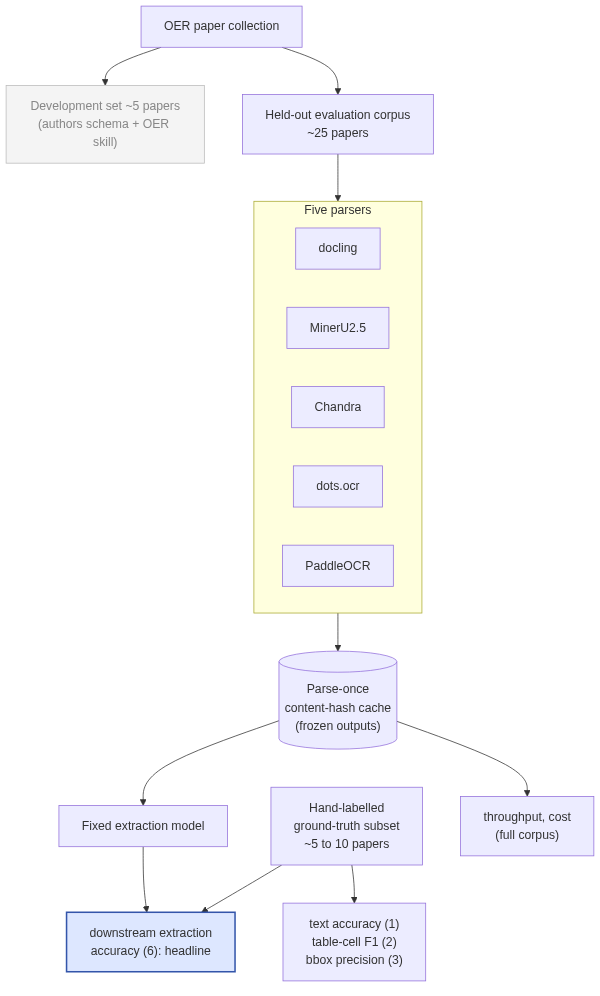
\includegraphics[width=0.62\textwidth]{eval-methodology.png}
    \caption{The parser-evaluation methodology. A development set authors the schema and skill; the held-out evaluation corpus is parsed by all five parsers into a frozen cache, and a fixed extraction model is applied. The accuracy metrics are scored against a hand-labelled subset. The apparatus is shown, not any results.}
    \label{fig:eval}
\end{figure}

\subsection{Schema strategy and skill-based extensibility}

The target schema can be obtained in two ways, which bracket the design space; we adopt a hybrid of them.

Under the \textbf{schema-first} strategy, the schema is authored in advance from domain knowledge: the classes (overpotential, Tafel slope, and so on), their units and ontology mappings, and the conditions each requires are defined, and the extraction model is then instructed to return data conforming to the schema, with every instance validated before it enters the graph. Its strengths are precision and interoperability, since each datum is typed, unit-bearing, and ontology-aligned on creation. Its weakness is rigidity: an unanticipated phenomenon has no place in the schema.

Under the \textbf{explore-first} strategy, the order is reversed: candidate fields are surfaced from the papers themselves and consolidated into a schema only afterwards. Its strength is coverage of unanticipated content. Its weakness is that, without control, it yields an inconsistent vocabulary and unvalidated data.

We adopt a schema-first core with an explore-first escape hatch. The authoritative schema is written in LinkML and generates the Pydantic models, validation shapes, and JSON-LD context used by the pipeline; extraction is validated against it, and only conforming instances are inserted. When the agent encounters a quantity or condition that the schema does not cover, such as a data point specific to one experiment or an additional figure of merit reported by a particular group, it neither discards the value silently nor alters the authoritative schema. Instead, it drafts a candidate field, presents it to the user, and records it in a separate exploratory schema file for review. Promotion from the exploratory file to the authoritative schema is an explicit manual decision.

This mechanism is also how a single corpus becomes a reusable asset, and how the system generalises beyond its demonstrator. A schema refined on one corpus serves as a template for the next: once the electrocatalysis vocabulary is stable, it provides the starting point for a related corpus, and the exploratory mechanism captures only the genuinely new fields the new corpus introduces.

Domain knowledge is packaged for the agent as a skill. Following the progressive-disclosure convention (Anthropic, 2025), a skill is a self-contained folder whose \texttt{SKILL.md} file contains a short YAML header, giving a name and a description of when the skill applies, followed by the domain instructions the agent requires: the quantities to extract, the conditions that qualify them, the unit conventions, and the common sources of error. Only the header resides in the agent's context by default; the body is loaded when the agent determines the skill to be relevant to the current paper. The electrocatalysis skill developed in this work is outlined below.

\begin{codebox}[code:skill]{The OER-extraction skill (outline)}{yaml}
---
name: oer-extraction
description: Extract OER / PEM-electrolysis figures of merit (overpotential,
  Tafel slope, exchange current density, ECSA, mass activity, TOF, stability)
  together with their measurement conditions. Use for acidic water-oxidation papers.
---

# What to extract
- Overpotential - always with its current density (10 mA cm-2 for RDE; 1-2 A cm-2 for cells)
- Tafel slope (mV/decade) - record the current-density range used for the fit
- Exchange current density, charge-transfer coefficient, ECSA, mass activity, turnover frequency
- Stability (hours) - with current density and cell type

# Conditions that qualify every measurement
- Electrolyte and pH, potential vs RHE, scan rate, temperature, cell type (RDE vs MEA)

# Traps
- Distinguish iR-corrected from uncorrected values, and record which.
- Do not conflate geometric and ECSA-normalised current density.
- A Tafel slope read off an LSV is not the same as one fitted over a stated range.
\end{codebox}

Authoring a skill for a new field follows the same hybrid path: the agent is directed at a sample of that field's papers, surfaces candidate quantities and conditions, consolidates them into a derived schema with ontology mappings, and writes the resulting heuristics and error cases into a new \texttt{SKILL.md}. The agent loop is unchanged; only the corpus, the schema, and one Markdown file differ. The durable output of this work is therefore not only an electrocatalysis knowledge graph but a documented method for converting a domain into a skill. The electrocatalysis skill is the first instance; the hydrogen-evolution reaction, CO$_2$ reduction, and other quantitative literatures would be added in the same manner, each as a separate skill rather than as a modification to the program. Extending the system therefore changes only the schema and the skill folder, never the agent loop.

\begin{figure}[H]
    \centering
    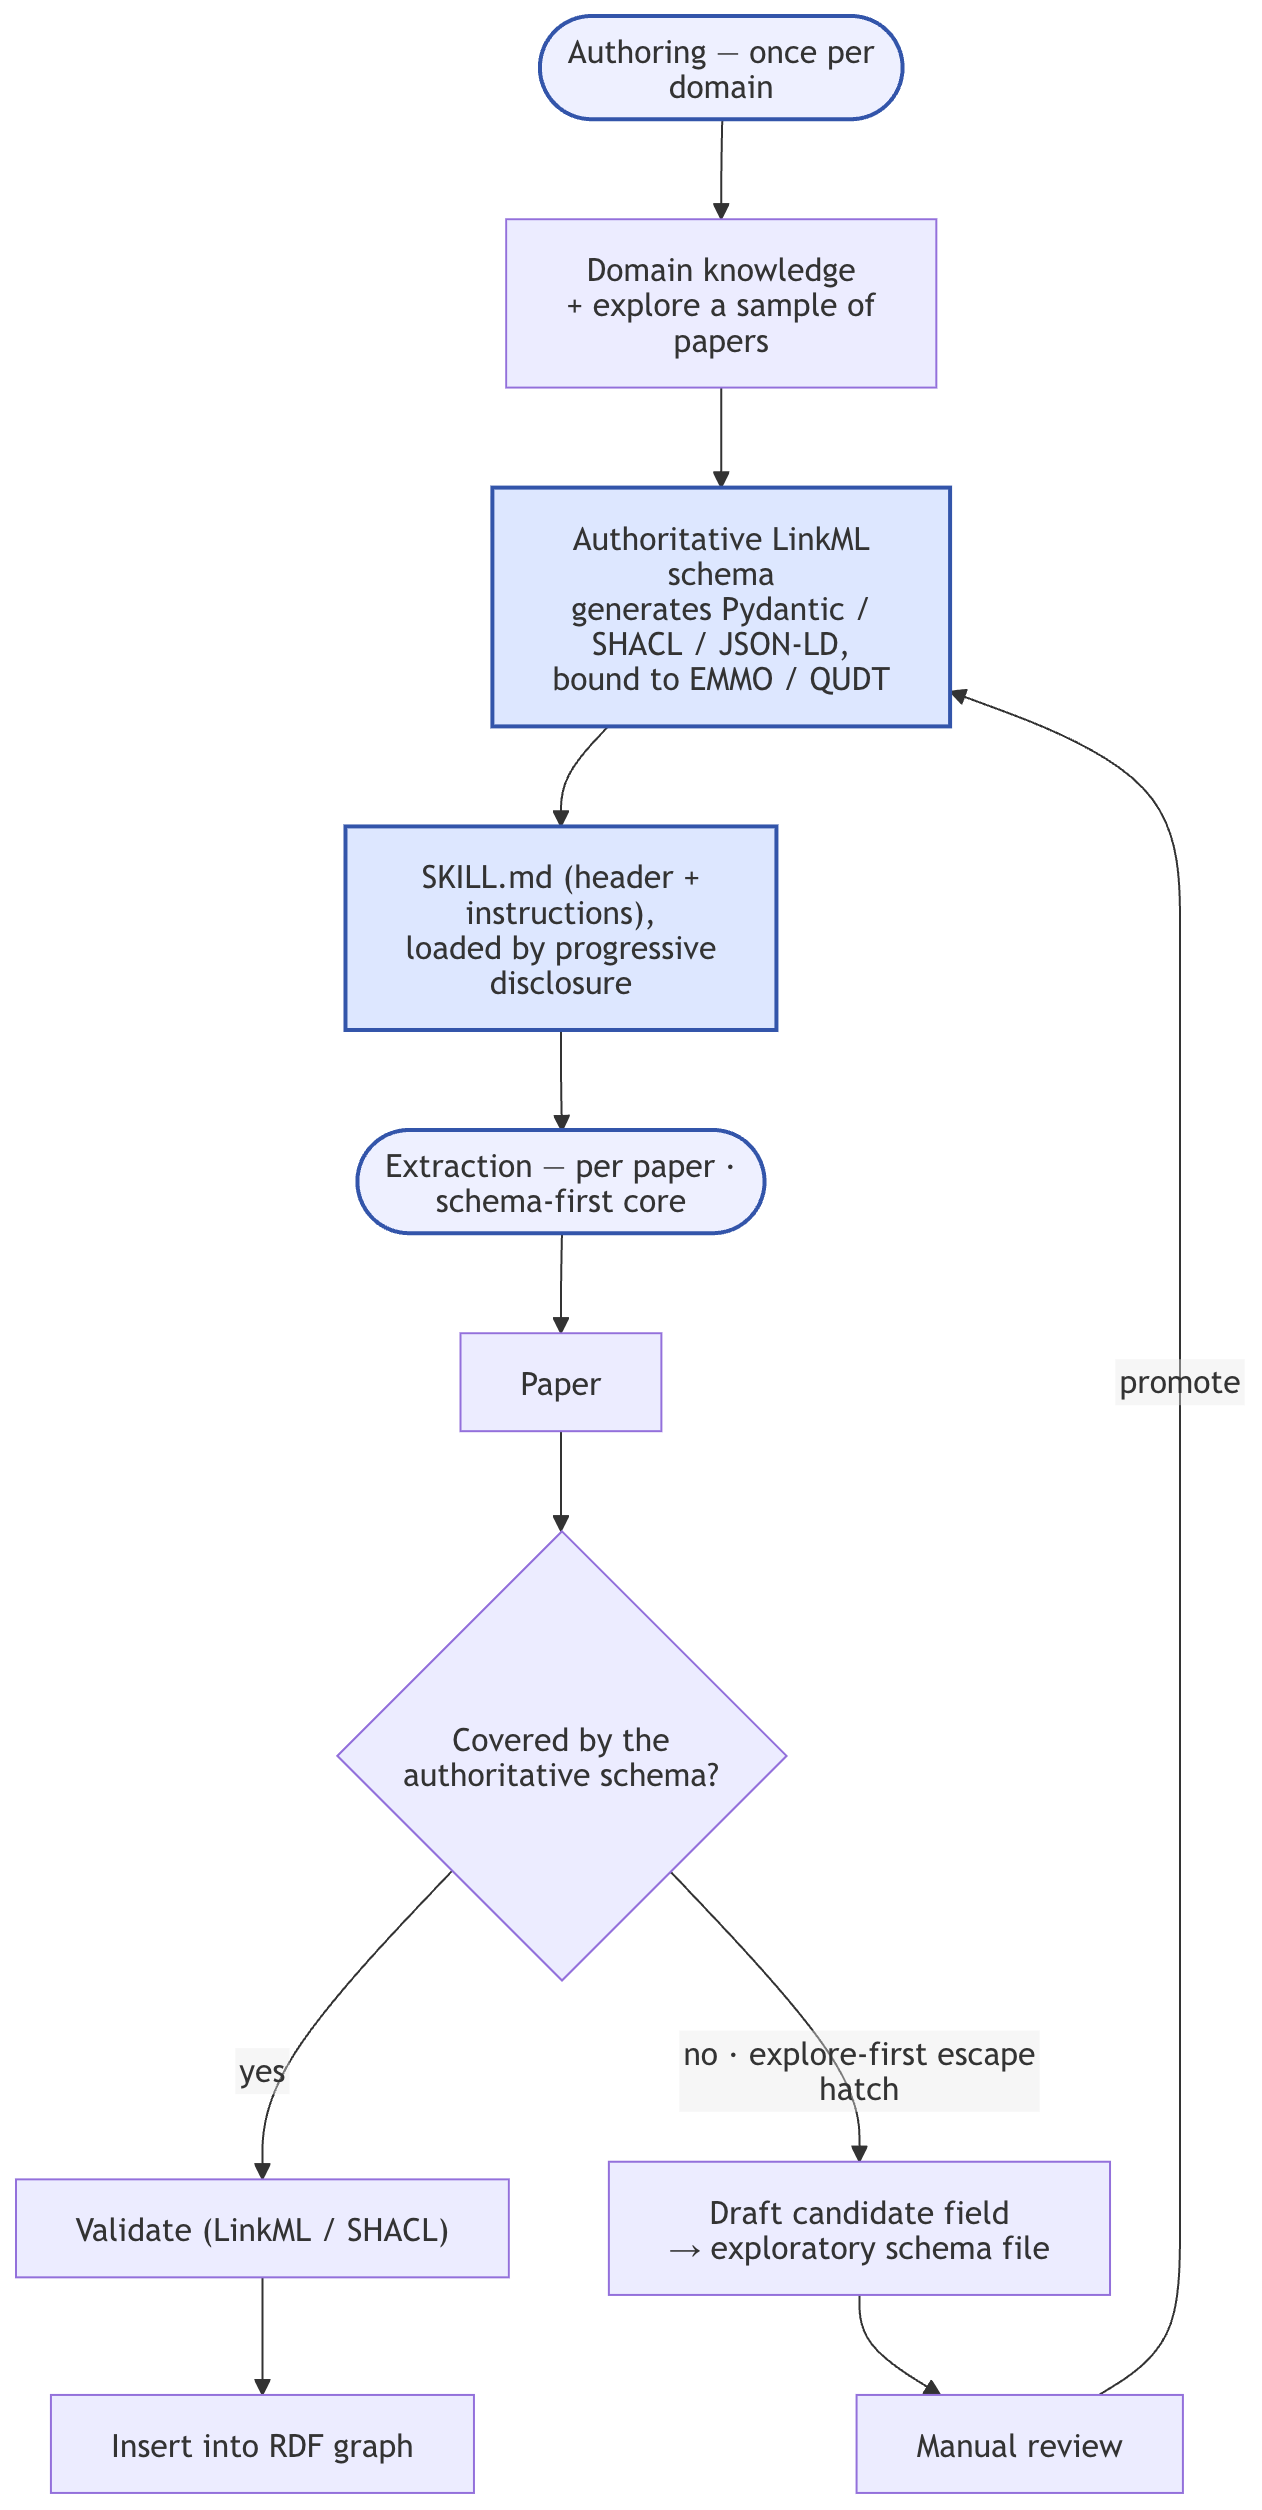
\includegraphics[width=0.5\textwidth]{skill-mechanism.png}
    \caption{Schema and skill mechanism, in two phases. A domain is authored once: an authoritative LinkML schema and its SKILL.md, built from domain knowledge and, for a genuinely new field, seeded by exploring a sample of its papers. Per paper, the schema-first core validates and inserts only measurements the schema covers; a value it does not cover is not dropped but drafted into an exploratory file for manual review and promotion back into the schema --- the explore-first escape hatch. The agent loop is unchanged; a new field is a new skill plus schema.}
    \label{fig:skill}
\end{figure}

\subsection{Ontology alignment and the EMMO gap}

Ontology alignment is a per-domain task performed at the schema level: each field binds its quantities to the established vocabularies that cover it, so a new domain reuses the same machinery against a different ontology without changes to the agent. For the electrocatalysis demonstrator, these vocabularies are the EMMO electrochemistry domain together with QUDT and PROV-O. Every slot in the schema carries an explicit ontology IRI. Where the EMMO electrochemistry domain defines a concept, such as overpotential, electrocatalyst, charge-transfer coefficient, the Butler--Volmer relation, or anodic reaction, we bind directly to the EMMO term (Del Nostro et al., 2024). Units bind to QUDT (QUDT, n.d.), and provenance binds to PROV-O (Lebo et al., 2013). Because units are resolved to QUDT and quantities to shared IRIs, a stored value can be consumed directly as a numerical parameter and compared across papers, rather than re-interpreted by hand at each downstream use.

The alignment also identifies a gap. Our review of the EMMO electrochemistry domain found two concepts central to OER work without direct counterparts. The first is the oxygen evolution reaction itself, for which the nearest available terms are more general, namely oxygen electrode, anodic reaction, and gas evolution. The second is the Tafel slope and Tafel equation, for which the closest kinetic-relation class is the Butler--Volmer equation. Rather than assign these to ill-fitting terms, we mint local IRIs under the palimpsest namespace and relate them to the nearest EMMO concept with \texttt{skos:closeMatch}, recording in the schema the additions that should be proposed to the ontology's maintainers. Pending confirmation against the published class index, we offer this as a reviewable list of OER concepts that would benefit from standardisation. A different field would align against a different part of EMMO, or against another community ontology; because this binding resides in the schema rather than in the agent, adding a domain does not affect the demonstrator's alignment.

\subsection{Provenance model}

Provenance in palimpsest is a precondition for inserting a datum, not metadata added afterwards. Every measurement inserted into the graph carries the source-paper hash, the parser that produced the text from which it was read, the page, the bounding box of the source region, and the extraction-run identifier, expressed as PROV-O activities and entities (Lebo et al., 2013). The operative rule is that a value which cannot be associated with its provenance is not inserted, and the failure is reported rather than suppressed. A value without a traceable origin is unsuitable, because it presents as authoritative while remaining unverifiable.

This discipline is what makes the resulting graph suitable to build upon. A query returns not only that a catalyst reaches a given overpotential at a given current density, but also which paper reported the value, which parser read it, and the location on the page from which it was extracted. This traceability is what allows a researcher to validate a value against its source before relying on it in a downstream decision, such as parameterising a simulation or selecting a candidate for synthesis, a check that matters because the extraction is automated and therefore fallible.

\begin{figure}[H]
    \centering
    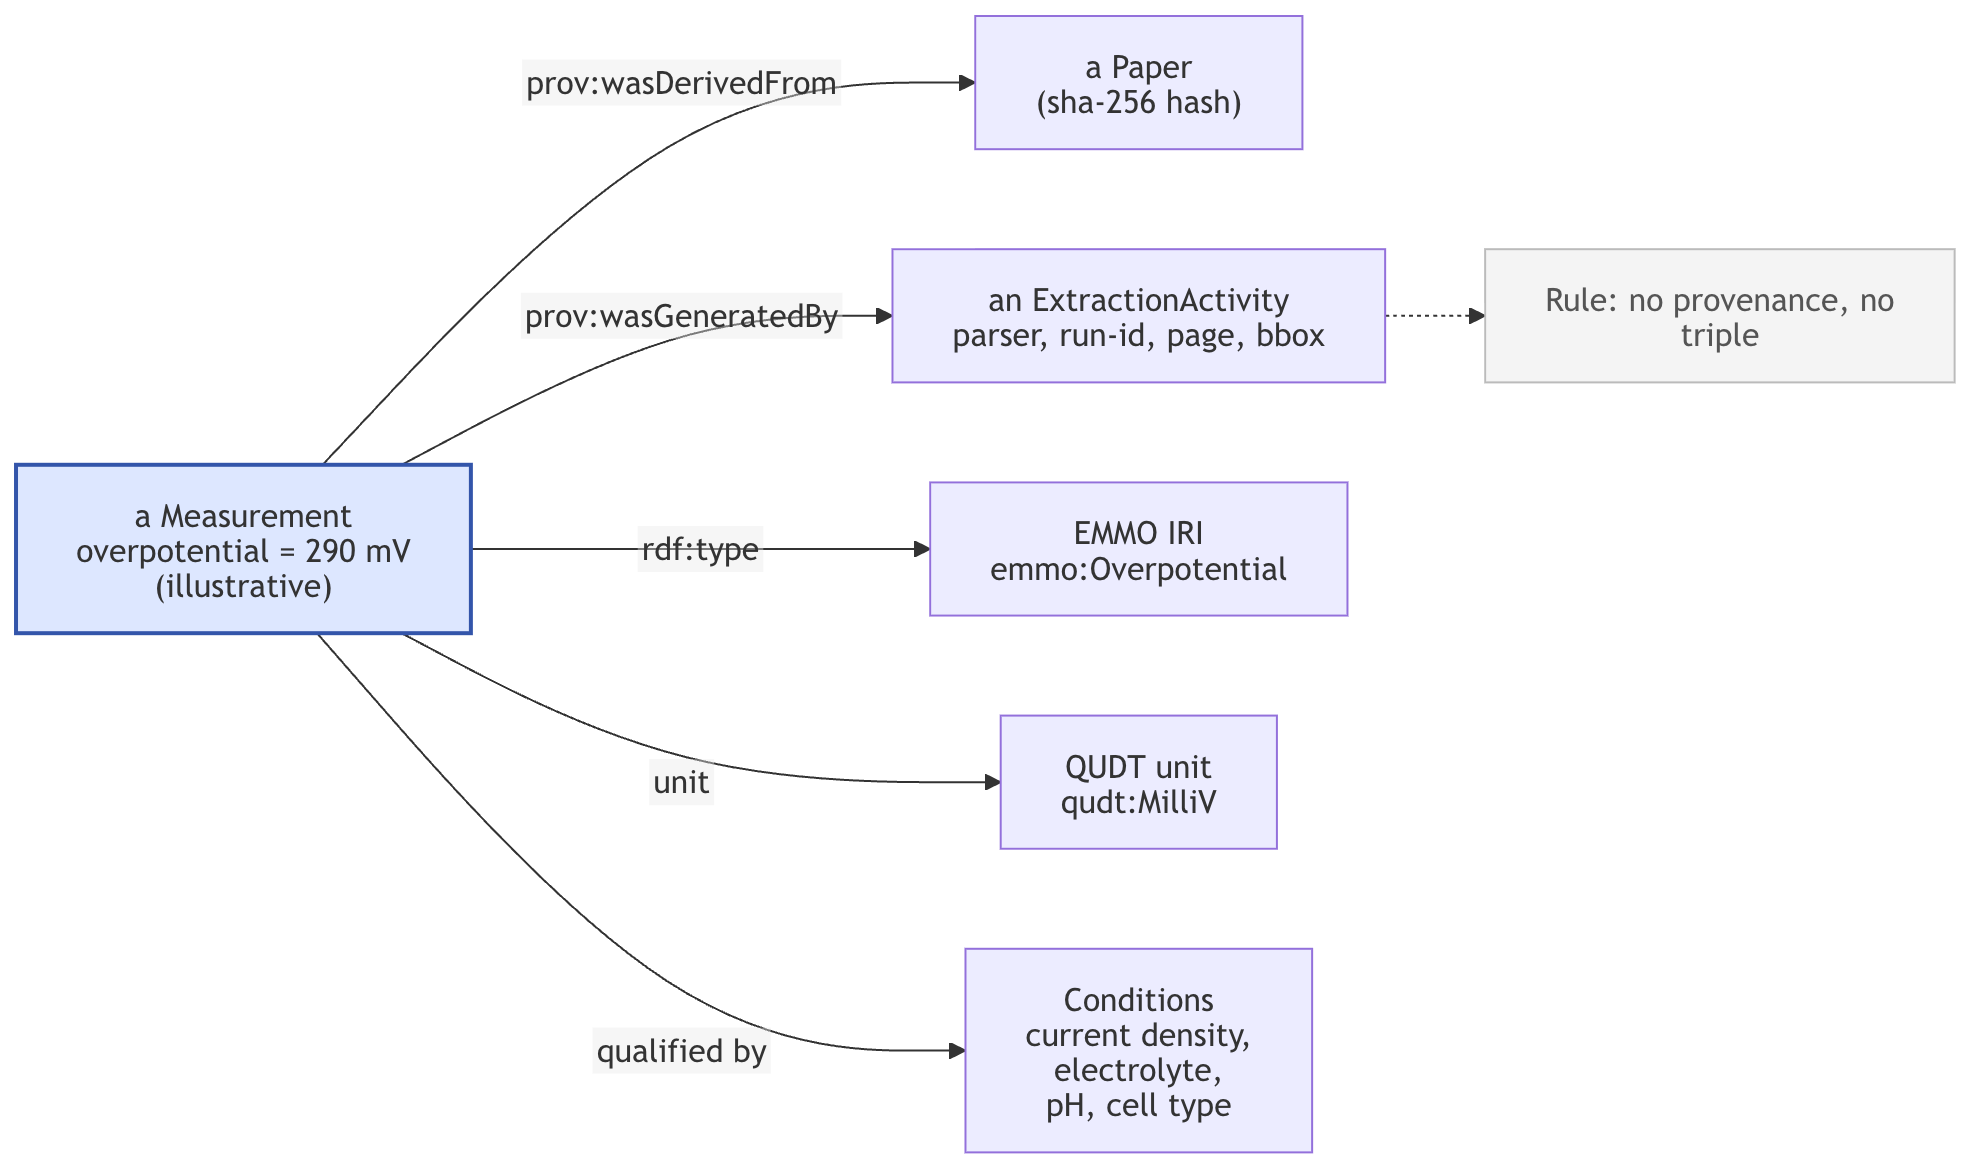
\includegraphics[width=0.9\textwidth]{provenance-model.png}
    \caption{The provenance data model. Each measurement is bound by PROV-O to its source paper and extraction activity (page, bbox, parser, run-id) and to EMMO and QUDT terms. The structure is shown with illustrative values; the graph is not populated here.}
    \label{fig:provenance}
\end{figure}

\subsection{Provenance viewer}

The provenance trail is usable only if it can be inspected directly, which is the function of the viewer: a single web page presenting the rendered PDF on the left and the extracted data on the right. Selecting a value highlights the region of the page from which it was extracted. The implementation is intentionally lightweight: a small server, a vendored PDF renderer, and hypermedia interactions rather than a single-page application. This is consistent with the overall minimalism of the system. Its purpose is verification: it makes provenance directly visible, which reduces the correction of an erroneous extraction to a brief inspection rather than a search through the source.

\subsection{Cost governance}

The agent incurs direct costs, for language-model calls and cloud GPUs, so cost is treated as a primary design concern. A cost meter records every paid call in a ledger and is consulted before each call. Spending is bounded by a fixed ceiling of \euro{}50, with graduated warnings as the total rises and refusal of any further API call once the ceiling is reached. The ceiling can be raised at run time through a slash command, but its default value is enforced. In combination with the parse-once cache, this keeps the study affordable and keeps its cost attributable: each amount is associated with a specific parse or extraction, which supports the reproducibility of the reported costs.

%--------------------------------------

\section{Current status}

The project is at an intermediate stage, and we state its status explicitly. The foundational infrastructure is implemented and has been exercised on real hardware: the five parsers are packaged and run on cloud GPUs, the GPU lifecycle and its cost accounting are implemented and verified, the parse-once content-hash cache is in place, and the agent loop, the primary model backend, and the cost meter are being implemented. The parser comparison is in progress on this foundation.

Several components that convert cached parser output into a validated, ontology-aligned graph are specified and under active development: the LinkML schema and its generated artefacts, the first domain skill (electrocatalysis), the extraction-and-validation step, the triple store with its provenance writes, and the viewer. Hand-labelled ground truth and the six evaluation metrics are the immediate next milestone. The apparatus that collects the raw material for the comparison is complete; the apparatus that scores it is under construction. No comparative results exist yet, and none are claimed.

%--------------------------------------

\section{Discussion}

\subsection{Hypotheses and expected outcomes}

The parser comparison is designed to answer a question that practitioners face but that the literature has not addressed for this domain: which document parser best enables a language model to recover electrocatalysis figures of merit, and at what cost and throughput. We state our expectations as two hypotheses, each tested by the metrics of Section 4.2.

\textbf{H1.} Transcription accuracy is a weak predictor of downstream extraction accuracy: the parser that maximises downstream accuracy (metric 6) will differ from the parser that maximises transcription accuracy (metric 1). This expectation follows from the second finding of Section 2.2, that extraction quality is bounded by the integrity of structured content rather than by aggregate text fidelity. We test H1 by comparing the two rankings on the hand-labelled subset and reject it if the same parser ranks first on both metrics. As a supporting descriptive measure, we report the Spearman rank correlation between the two orderings, which we expect to be low. Given the small number of parsers (n = 5), this correlation is reported descriptively rather than as a significance test.

\textbf{H2.} Parsers that preserve table structure faithfully will yield higher downstream accuracy on this corpus than parsers with higher aggregate text fidelity but weaker table recovery, because the figures of merit in OER papers are concentrated in tables. We test H2 by relating per-parser table-cell F1 (metric 2) to downstream accuracy (metric 6), expecting a positive rank association, which we report descriptively given n = 5, as for H1. Because metric (6) is computed partly over table-bound quantities, a positive association is in part expected by construction; H2 is therefore informative chiefly through its failure modes, and would be contradicted by a parser with high table-cell F1 but low downstream accuracy, for instance one that recovers table structure yet misreads units or the cells carrying the qualifying conditions.

The magnitude of these effects, if present, is the empirical contribution of the study. The result is also of practical use: it indicates, for this literature, which parser to adopt and on what basis. Because the comparison method is domain-general, the same procedure applied to another field's corpus would address the same question there; the electrocatalysis result, once produced, will be the first such data point rather than a general conclusion.

\subsection{Significance}

Several design choices combine to give the system the following properties.

The data the system produces will be FAIR by construction (Wilkinson et al., 2016): each datum is findable in a queryable graph, interoperable through EMMO and QUDT alignment, and reusable because it is typed, unit-bearing, and provenance-complete. The provenance discipline makes the graph auditable, which is relevant because language-model extraction is fallible. The parse-once cache makes the comparison reproducible, since every parser is evaluated on identical frozen inputs. The minimal, framework-free architecture keeps the system legible and modifiable. The interchangeable model backends, together with a fixed budget, make running costs controllable and transparent. Under skill-based extensibility, domain knowledge is held in a \texttt{SKILL.md} file and a schema rather than in the agent, so a new field is added as a new skill rather than as new code. We demonstrate how a domain is added, with electrocatalysis as the worked instance, and claim nothing about fields not yet attempted.

Taken together, traceability, low cost, reproducibility, and extensibility are the properties expected of research infrastructure, with the OER ontology-gap analysis of Section 4.4 as an additional output that contributes to the broader materials-ontology effort.

More broadly, the system is positioned as the data layer of a data-driven materials-design workflow. Extraction is the first stage of a longer process in which curated values are assessed for relevance and reliability, then used as parameters for simulation or as priors for selecting experiments, with results feeding back into the graph (de Pablo et al., 2019; Abolhasani \& Kumacheva, 2023). The properties above are what make the extracted data usable at that next stage rather than merely stored: unit normalisation makes values directly consumable as parameters, the schema and ontology make them categorisable and queryable, and provenance lets a researcher verify a value against its source before committing it to a costly simulation or experiment. Palimpsest performs the extraction and curation stage only. The analysis, simulation, and experimental selection it is intended to support lie outside the scope of this work and are noted as future work in Section 7.

\subsection{Limitations}

Several limitations bound the claims this study can support. The evaluation corpus is modest, about 25 papers from the single narrow domain of acidic OER and PEM electrolysis, and the accuracy metrics rest on a smaller hand-labelled subset of it. This makes reliable extraction and meaningful ontology alignment tractable at this scale, but it also means the parser ranking should be interpreted as specific to dense, table-heavy electrochemistry papers and not assumed to transfer to other literatures. The downstream-accuracy results are obtained with a single extraction model. A different model could reorder the parsers, and the sensitivity of the ranking to model choice is outside the present scope. Ground-truth labelling is manual and therefore limited in volume, which constrains the statistical strength of the comparison. The study is best characterised as a controlled case study rather than a large-scale benchmark. The practical handling of both the single-model dependence and the labelling effort is described as risks in Section 6.4; here we note only their effect on the claims the study can support. The ontology alignment depends on the current state of EMMO, and the local IRIs minted for OER and Tafel concepts are an interim measure pending standardisation. Finally, generality is established by construction on a single demonstrator: the architecture reduces the addition of a domain to authoring a skill, but this has so far been exercised on one field, and validating it on a second domain end to end remains future work.

\subsection{Risks, challenges, and mitigations}

Beyond the limitations on what may be claimed, the project has encountered, and anticipates, a number of engineering and methodological challenges. Table 2 records the principal ones, their current status, and the corresponding mitigation or resolution plan. We distinguish challenges already encountered (\textit{faced}), those expected as the work proceeds (\textit{anticipated}), and those that are continuous (\textit{ongoing}).

{\small
\begin{longtable}{@{}>{\raggedright\arraybackslash}p{4.2cm} >{\raggedright\arraybackslash}p{2.2cm} >{\raggedright\arraybackslash}p{8.0cm}@{}}
\caption{Principal risks and challenges, their status, and the corresponding mitigations.}\label{tab:risks}\\
\toprule
\textbf{Risk / challenge} & \textbf{Status} & \textbf{Mitigation / resolution plan} \\
\midrule
\endfirsthead
\multicolumn{3}{l}{\itshape\small Table 2 (continued)}\\
\toprule
\textbf{Risk / challenge} & \textbf{Status} & \textbf{Mitigation / resolution plan} \\
\midrule
\endhead
\midrule
\multicolumn{3}{r}{\itshape\small continued on next page}\\
\endfoot
\bottomrule
\endlastfoot
GPU-capacity scarcity and price variability on community cloud & Faced & Request GPU types cheapest-first with automatic fallback; use RunPod.io secure-cloud instances when community capacity is unavailable; retain a third-party provider (Vast.ai) as a further fallback. \\
\addlinespace
Conflicting dependency stacks across parsers (runtime and framework pins) & Faced & Package each parser in its own isolated container image; do not co-locate parsers in a single environment. \\
\addlinespace
Vendor parser image not self-controllable (olmOCR: FP8/Ada-only, no SSH access) & Faced & Exclude olmOCR; add dots.ocr and PaddleOCR to preserve five parsers across three design families. \\
\addlinespace
Ground-truth labelling cost and subjectivity & Ongoing & Label a small reference subset under a documented protocol; record annotator decisions; report the study as a controlled case study rather than a benchmark. \\
\addlinespace
Dependence on a single extraction model for downstream accuracy & Anticipated & Hold the model and prompt fixed for comparability; record model and version with every run; treat cross-model sensitivity as defined future work. \\
\addlinespace
Non-determinism in re-parsing confounding the comparison & Faced & Parse each (paper, parser) pair once and cache by content hash; compute all metrics on the frozen outputs. \\
\addlinespace
Language-model extraction errors and hallucinated values & Anticipated & Constrain extraction to the schema and validate with SHACL; apply a conversational re-query and rejection step (cf. Polak \& Morgan, 2024); insert only validated instances. \\
\addlinespace
Values without traceable provenance entering the graph & Faced (by design) & Enforce the rule that a triple lacking complete provenance is not inserted and the failure is reported. \\
\addlinespace
Parsers that do not emit element-level bounding boxes & Anticipated & Score bounding-box availability and precision as an explicit metric; have the viewer highlight at coarser granularity where element boxes are absent. \\
\addlinespace
Missing EMMO terms for OER and Tafel concepts & Faced & Mint local IRIs with \texttt{skos:closeMatch} to the nearest EMMO concept; document the proposed additions for the ontology maintainers. \\
\addlinespace
Fixed \euro{}50 operating budget (for parsing only) & Faced & Check the cost meter before each paid call; rely on the parse-once cache to avoid repeated costs; apply graduated warnings and a hard stop at the ceiling. \\
\end{longtable}
}

%--------------------------------------

\section{Conclusion}

Palimpsest addresses a general problem: the quantitative content of the scientific literature is held in PDFs in a form that machines cannot reuse. The system reads this literature using interchangeable state-of-the-art parsers and extracts the quantities relevant to a field, specified by a skill rather than encoded in the agent. It aligns them to established ontologies for the field, its units, and its provenance, and records the origin of each value to the level of the page region from which it was read. We develop and evaluate the system on energy-materials electrocatalysis, where our first empirical contribution is to treat the parser as an experimental variable and to measure downstream extraction accuracy: whether a language model recovers the intended measurement from each parser's output. The infrastructure for this comparison is implemented and the study is in progress. The schema, extraction, and viewer components that complete the pipeline are specified and under development. The same machinery, extended by an additional skill, supports application to further domains. Beyond extraction, the curated graph is intended to serve the downstream stages of a data-driven design workflow: assessing which data are reliable and comparable, supplying parameters to simulations, and helping prioritise experiments in a closed loop with prediction (Abolhasani \& Kumacheva, 2023). These stages are enabled by, but not performed in, the present work. The remaining work is to produce and score the comparison results and to author the next skill, which forms the basis of the subsequent chapters.

%--------------------------------------

\section*{References}
\addcontentsline{toc}{section}{References}

\begingroup
\setlength{\parindent}{0pt}
\setlength{\parskip}{0.5em}
\everypar{\hangindent=1.5em \hangafter=1}

Abolhasani, M., \& Kumacheva, E. (2023). The rise of self-driving labs in chemical and materials sciences. \textit{Nature Synthesis}, 2, 483--492. \url{https://doi.org/10.1038/s44160-022-00231-0}

Anthropic (2025). \textit{Equipping agents for the real world with Agent Skills}. Anthropic Engineering, 16 October 2025. \url{https://www.anthropic.com/engineering/equipping-agents-for-the-real-world-with-agent-skills}

Auer, C., Lysak, M., Nassar, A., Dolfi, M., Livathinos, N., Vagenas, P., Berrospi Ramis, C., Omenetti, M., Lindlbauer, F., Dinkla, K., Mishra, L., Kim, Y., Gupta, S., Teixeira de Lima, R., Weber, V., Morin, L., Meijer, I., Kuropiatnyk, V., \& Staar, P. W. J. (2024). \textit{Docling Technical Report}. arXiv:2408.09869.

Ball, T. (2025). \textit{How to Build an Agent}. ampcode.com, 15 April 2025. \url{https://ampcode.com/how-to-build-an-agent}

Butler, K. T., Davies, D. W., Cartwright, H., Isayev, O., \& Walsh, A. (2018). Machine learning for molecular and materials science. \textit{Nature}, 559(7715), 547--555. \url{https://doi.org/10.1038/s41586-018-0337-2}

Carmo, M., Fritz, D. L., Mergel, J., \& Stolten, D. (2013). A comprehensive review on PEM water electrolysis. \textit{International Journal of Hydrogen Energy}, 38(12), 4901--4934. \url{https://doi.org/10.1016/j.ijhydene.2013.01.151}

Datalab (2026). \textit{Chandra: an OCR model for complex tables, forms, and handwriting with full layout} [software]. \url{https://github.com/datalab-to/chandra}

de Pablo, J. J., Jackson, N. E., Webb, M. A., Chen, L.-Q., Moore, J. E., Morgan, D., Jacobs, R., Pollock, T. M., Schlom, D. G., Toberer, E. S., et al. (2019). New frontiers for the materials genome initiative. \textit{npj Computational Materials}, 5, 41. \url{https://doi.org/10.1038/s41524-019-0173-4}

Del Nostro, P., Friis, J., Ghedini, E., Goldbeck, G., Holtz, O., Roscioni, O. M., Zaccarini, F. A., \& Toti, D. (2024). Elementary Multiperspective Material Ontology: Leveraging Perspectives via a Showcase of EMMO-Based Domain and Application Ontologies. In \textit{Proceedings of the 16th International Joint Conference on Knowledge Discovery, Knowledge Engineering and Knowledge Management (IC3K 2024) - Volume 2: KEOD} (pp. 135--142). SciTePress.

Dunn, A., Dagdelen, J., Walker, N., Lee, S., Rosen, A. S., Ceder, G., Persson, K., \& Jain, A. (2022). \textit{Structured information extraction from complex scientific text with fine-tuned large language models}. arXiv:2212.05238.

Lebo, T., Sahoo, S., McGuinness, D., Belhajjame, K., Cheney, J., Corsar, D., Garijo, D., Soiland-Reyes, S., Zednik, S., \& Zhao, J. (2013). \textit{PROV-O: The PROV Ontology}. W3C Recommendation, 30 April 2013. \url{https://www.w3.org/TR/prov-o/}

McCrory, C. C. L., Jung, S., Peters, J. C., \& Jaramillo, T. F. (2013). Benchmarking heterogeneous electrocatalysts for the oxygen evolution reaction. \textit{Journal of the American Chemical Society}, 135(45), 16977--16987. \url{https://doi.org/10.1021/ja407115p}

Moxon, S., Solbrig, H., Unni, D., Jiao, D., Bruskiewich, R., Balhoff, J., Vaidya, G., Duncan, W., Hegde, H., Miller, M., Brush, M., Harris, N., Haendel, M., \& Mungall, C. (2021). The Linked Data Modeling Language (LinkML): A General-Purpose Data Modeling Framework Grounded in Machine-Readable Semantics. \textit{CEUR Workshop Proceedings}, Vol. 3073, 148--151.

Niu, J., et al. (2025). \textit{MinerU2.5: A Decoupled Vision-Language Model for Efficient High-Resolution Document Parsing}. arXiv:2509.22186.

PaddleOCR Team, Baidu Inc. (2025). \textit{PaddleOCR 3.0 Technical Report}. arXiv:2507.05595.

Polak, M. P., \& Morgan, D. (2024). Extracting accurate materials data from research papers with conversational language models and prompt engineering. \textit{Nature Communications}, 15, 1569. \url{https://doi.org/10.1038/s41467-024-45914-8}

Poznanski, J., Rangapur, A., Borchardt, J., Dunkelberger, J., Huff, R., Lin, D., Wilhelm, C., Lo, K., \& Soldaini, L. (2025). \textit{olmOCR: Unlocking Trillions of Tokens in PDFs with Vision Language Models}. arXiv:2502.18443.

QUDT (n.d.). \textit{QUDT - Quantities, Units, Dimensions and Types} [ontology]. Accessed May 2026. \url{https://www.qudt.org/}

rednote-hilab (2025). \textit{dots.ocr: multilingual document layout parsing in a single vision-language model} [software]. \url{https://github.com/rednote-hilab/dots.ocr}

Wilkinson, M. D., Dumontier, M., Aalbersberg, I. J., Appleton, G., Axton, M., Baak, A., et al. (2016). The FAIR Guiding Principles for scientific data management and stewardship. \textit{Scientific Data}, 3, 160018. \url{https://doi.org/10.1038/sdata.2016.18}

\endgroup

\end{document}
